% !TEX program = lualatex
\documentclass[10pt]{beamer}

\usetheme[progressbar=frametitle]{metropolis}
\usepackage{appendixnumberbeamer}

\usepackage{graphicx}
\usepackage{booktabs}
\usepackage{colortbl}
\usepackage[scale=2]{ccicons}

\usepackage{braket}

\usepackage{pgfplots}
\usepgfplotslibrary{dateplot}
\usepackage[font=scriptsize,labelfont=bf]{caption}

\usepackage{tikz}
\usetikzlibrary{fit,shapes,positioning,calc,shapes.geometric,backgrounds}
\colorlet{tempGray}{gray!80!cyan}
\colorlet{lightgray}{tempGray!60!white}
\colorlet{orange}{red!30!yellow}
\colorlet{lightorange}{orange!60!white}
\colorlet{darkGreen}{green!80!black}
\colorlet{paleGreen}{darkGreen!30!white}

\tikzset{
  invisible/.style={opacity=0, text opacity=0},
  visible on/.style={alt={#1{}{invisible}}},
  alt/.code args={<#1>#2#3}{\alt<#1>{\pgfkeysalso{#2}}{\pgfkeysalso{#3}}},
}

\usepackage{xspace}
\newcommand{\themename}{\textbf{\textsc{metropolis}}\xspace}


\def\code#1{\texttt{#1}}
\newcommand{\lighthline}{\arrayrulecolor{gray!35}\hline\arrayrulecolor{black}}

\title{Quantum Memories via Microwave Electron Spin Ensembles}
\author{Linus Kelsey}
\date{21 Jul 26}
\institute{UCL Department of Physics and Astronomy}

\begin{document}

\maketitle

% MOTIVATION =================================================
\begin{frame}{Why Quantum Memories?}
    \textbf{The Scale Problem:} Fault-tolerant QC demands unscalable physical footprint
    \begin{center}
    \scalebox{0.82}{%
        \begin{tikzpicture}
            \node[draw, fill=lightgray, minimum width=3.0cm, minimum height=1.6cm, align=center, visible on=<1->] at (0,0)
                {RSA-2048 via\\Shor's algo\\$\sim$ 1M qubits\\{\scriptsize (Gidney, 2025)}};
            \node[draw, fill=lightorange, minimum width=3.0cm, minimum height=1.6cm, align=center, visible on=<2->] at (4.5,0)
                {Monolithic chip:\\13M qubits \Rightarrow\\$5\times5$\,m footprint\\{\scriptsize (Alexander, 2023)}};
            \node[draw, fill=paleGreen, minimum width=3.0cm, minimum height=1.6cm, align=center, visible on=<3->] at (9,0)
                {\textbf{With memory:}\\Shor's just\\13,436 qubits\\{\scriptsize (Gouzien \& Sangouard, 2021)}};
        \end{tikzpicture}%
    }
    \end{center}
    \begin{uncoverenv}<3->
    Quantum memory offloads intermediate states from processor, amortises qubit overhead across time

    Gouzien \& Sangouard's result requires multimode storage times no shorter than $\sim$ 1s

    \textbf{Microwave regime} necessary for superconducting compatibility
    \end{uncoverenv}
\end{frame}

% PLATFORM ===================================================
\begin{frame}{Spin Ensemble Platform}
    \textbf{Key physics:} spin ensemble coupled to microwave cavity via collective coupling $g_\mathrm{eff} = g_0\sqrt{N}$
    \begin{itemize}
        \item<1-> Hz-scale $g_0$ $\to$ MHz-scale $g_\mathrm{eff}$ at modest $N\sim10^{12}$ spins
        \item<2-> Strong coupling in ensemble inaccessible to single spins
        \item<3-> \textbf{Cooperativity} $C = g_\mathrm{eff}^2/(\kappa\gamma)$: spin-cavity efficiency $= 4C/(1+C)^2$, maximised at $C = 1$
    \end{itemize}
    \vspace{0.1cm}
    \begin{uncoverenv}<4->
    \textbf{Material platforms:}
    \begin{center}
    \scriptsize
    \renewcommand{\arraystretch}{1.2}
    \begin{tabular}{lll}
        \toprule
        \textbf{System} & \textbf{Key property} & \textbf{Role} \\
        \midrule
        Si:Bi & Rich hyperfine manifold, microwave transitions & Primary memory \\
        \lighthline
        NV/diamond & First coupling of ensemble and SC qubit & Proof of concept \\
        \lighthline
        Yb:YSO & $C\geq1$; microwave transitions at zero field & High-$C$ platform \\
        \lighthline
        Er$^{3+}$:CaWO$_4$ & Telecom-band optical transitions & Network bridge \\
        \bottomrule
    \end{tabular}
    \end{center}
    \end{uncoverenv}
\end{frame}

% COHERENCE + CLOCK TRANSITIONS =============================
\begin{frame}{Coherence Engineering: Clock Transitions}
  \textbf{Challenge:} inhomogeneous broadening spreads spin resonances; \textit{ensemble dephases} faster than spins decohere

    \vspace{0.15cm}
    \textbf{Clock transitions}: frequencies insensitive to magnetic field fluctuations (\emph{1st order}), dominant noise channel suppressed

    \vspace{0.15cm}
  \textbf{Si:Bi}: hyperfine structure gives clock transitions in the superconducting qubit band

    \vspace{0.1cm}
    \begin{uncoverenv}<2->
    \begin{center}
    \scalebox{0.75}{%
    \begin{tikzpicture}[
      sp/.style={->, thick},
      axline/.style={-latex, thick, gray!60}
    ]

    %% LEFT PANEL: clock transition ω vs B
    \draw[axline] (-0.15,0) -- (4.4,0) node[right, font=\tiny, gray!70] {$B$};
    \draw[axline] (0,-0.15) -- (0,1.55) node[above, font=\tiny, gray!70] {$\omega/2\pi$};

    % Transition frequency curve: ω = 0.25 + 0.28*(B-2)^2
    \draw[thick, teal!70!black, domain=0:4, smooth, samples=60]
      plot (\x, {0.25 + 0.28*(\x-2)*(\x-2)});

    % Clock point at B=2, ω=0.25
    \filldraw[teal!70!black] (2,0.25) circle (1.5pt);

    % Horizontal tangent at clock
    \draw[dashed, teal!55!black, thick] (1.2,0.25) -- (2.8,0.25);
    \node[font=\tiny, teal!70!black, anchor=south] at (2,0.32)
      {$\tfrac{\mathrm{d}\omega}{\mathrm{d}B}{=}0$};

    % Label arrow
    \draw[->, gray!60, thin] (3.3,1.1) -- (2.1,0.30);
    \node[font=\scriptsize, gray!55, anchor=west] at (2.9,1.3) {clock};

    \node[font=\tiny, gray!60, align=center, anchor=north] at (2,-0.55)
      {Clock transition: $\mathrm{d}\omega/\mathrm{d}B{=}0$ cancels field-noise dephasing};

    %% RIGHT PANEL: T₂ log-scale bars
    %% 1 µs (x=0) to 10 s (x=5 cm), 7 decades, 5/7 cm per decade
    \begin{scope}[xshift=6.5cm, yshift=0cm]
      \draw[axline] (-0.05,0) -- (5.35,0);
      \node[below right, font=\tiny, gray!70] at (5.35,-0.08) {time (log scale)};

      % Tick: 1 µs at x=0
      \draw (0,0.07) -- (0,-0.07);
      \node[below, font=\tiny] at (0,-0.10) {$1\,\mu$s};
      % Tick: 1 ms at x = 3*(5/7) = 2.143
      \draw (2.143,0.07) -- (2.143,-0.07);
      \node[below, font=\tiny] at (2.143,-0.10) {1\,ms};
      % Tick: 1 s at x = 6*(5/7) = 4.286
      \draw (4.286,0.07) -- (4.286,-0.07);
      \node[below, font=\tiny] at (4.286,-0.10) {1\,s};

      % T₂* ~10 µs: 1 decade → x = 0.714
      \fill[red!45] (0,0.42) rectangle (0.714,0.63);
      \draw[red!60!black, thick] (0.714,0.11) -- (0.714,-0.11);
      \node[below, font=\tiny, red!70!black] at (0.714,-0.13) {${\sim}\mu$s};
      \node[right, font=\scriptsize] at (0.73,0.525) {$T_2^*$ (Si:Bi)};

      % T₂ natural Si:Bi = 93 ms: log₁₀(0.093)≈−1.03, offset 4.97 decades → x = 3.549
      \fill[orange!55] (0,0.80) rectangle (3.549,1.01);
      \draw[orange!70!black, thick] (3.549,0.11) -- (3.549,-0.11);
      \node[below, font=\tiny, orange!70!black] at (3.549,-0.13) {93\,ms};
      \node[right, font=\scriptsize] at (3.56,0.905) {nat.\ Si:Bi};

      % T₂ clock ²⁸Si:Bi = 2.7 s: log₁₀(2.7)≈0.43, offset 6.43 decades → x = 4.594
      \fill[darkGreen!55] (0,1.19) rectangle (4.594,1.40);
      \draw[darkGreen!80!black, thick] (4.594,0.11) -- (4.594,-0.11);
      \node[below, font=\tiny, darkGreen!80!black] at (4.594,-0.13) {2.7\,s};
      \node[right, font=\scriptsize] at (4.60,1.295) {$^{28}$Si:Bi clock};

      \node[font=\tiny, gray!65, anchor=north] at (2.5,-0.55) {Intrinsic coherence times $T_2$, $T_2^*$ from \textit{Wolfowicz et al.\ (2013)}};
    \end{scope}

    \end{tikzpicture}%
    }
    \end{center}
    \end{uncoverenv}
\end{frame}

% HYBRID ARCHITECTURE ========================================
\begin{frame}{Hybrid Architecture and Proof of Concept}
    Two milestones bridge SC-spin coupling to operational memory:
    \begin{itemize}
        \item<1-> SC qubit state coherently mapped into spin ensemble and retrieved (Kubo \textit{et al.}, 2011): hybrid architecture validated
    \end{itemize}

    \begin{center}
        {\setlength{\fboxrule}{0.5pt}\setlength{\fboxsep}{0pt}%
        \textcolor{gray!80}{\fbox{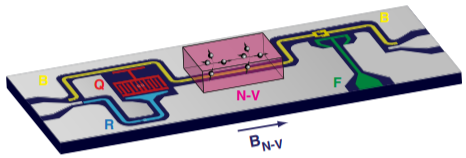
\includegraphics[width=0.55\linewidth]{../artefacts/img/kubo_nv_memory.png}}}}\\[2pt]
        {\tiny\textit{Kubo et al.\ (2011): transmon qubit Q coupled to NV/diamond spin ensemble via microwave bus B}}
    \end{center}

    \vspace{-6pt}
    \begin{itemize}
        \item<2-> Clock-transition-enabled storage in Si:Bi: first solid-state multimode microwave QM (Ranjan \textit{et al.}, 2020), 100\,ms storage
        \item<3-> Hahn echo commits to fixed retrieval order (FILO) and population inversion causes ASE noise
    \end{itemize}
\end{frame}

% WURST ======================================================
\begin{frame}[t]{Random-Access Protocol: WURST Pulses}
    \small Chirped $\pi$-pulse pairs imprint unique phase labels $\phi_W$; each label selects a stored mode for readout - giving random access without population inversion
    \begin{center}
    \scalebox{0.50}{%
    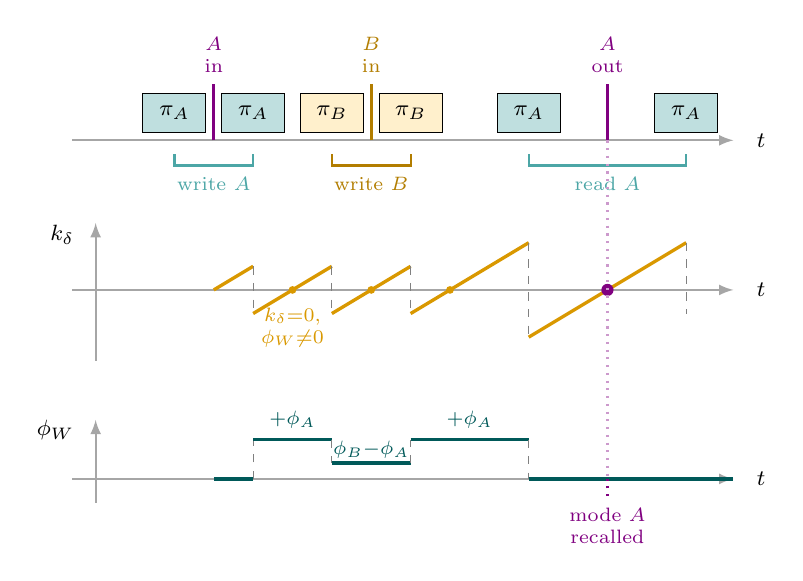
\begin{tikzpicture}[
      font=\footnotesize,
      wurst/.style={draw, fill=teal!25, minimum width=8mm, minimum height=5mm, inner sep=1pt},
      wurstB/.style={draw, fill=orange!20, minimum width=8mm, minimum height=5mm, inner sep=1pt},
      axline/.style={-latex, thick, gray!70},
    ]
    \def\T{8.1}
    \def\tW{1.0}
    \def\tE{1.5}
    \def\tWb{2.0}
    \def\tB{3.0}
    \def\tBe{3.5}
    \def\tBb{4.0}
    \def\tR{5.5}
    \def\tEcho{6.5}
    \def\tRb{7.5}

    % ROW 1: pulse sequence
    \begin{scope}[yshift=0cm]
      \draw[axline] (-0.3,0) -- (\T,0);
      \node at (\T+0.35,0) {$t$};
      % write A (slide 1+)
      \node[wurst, visible on=<1->]  at (\tW, 0.35) {$\pi_A$};
      \draw[very thick, violet, visible on=<1->] (\tE,0) -- (\tE,0.72);
      \node[violet, anchor=south, align=center, font=\scriptsize, visible on=<1->] at (\tE,0.74) {$A$\\in};
      \node[wurst, visible on=<1->]  at (\tWb,0.35) {$\pi_A$};
      \draw[teal!70, thick, visible on=<1->] (\tW,-0.18) -- (\tW,-0.32) -- (\tWb,-0.32) -- (\tWb,-0.18);
      \node[teal!70, font=\scriptsize, anchor=north, visible on=<1->] at ({(\tW+\tWb)/2},-0.34) {write $A$};
      % write B (slide 2+)
      \node[wurstB, visible on=<2->] at (\tB, 0.35) {$\pi_B$};
      \draw[very thick, orange!70!black, visible on=<2->] (\tBe,0) -- (\tBe,0.72);
      \node[orange!70!black, anchor=south, align=center, font=\scriptsize, visible on=<2->] at (\tBe,0.74) {$B$\\in};
      \node[wurstB, visible on=<2->] at (\tBb,0.35) {$\pi_B$};
      \draw[orange!70!black, thick, visible on=<2->] (\tB,-0.18) -- (\tB,-0.32) -- (\tBb,-0.32) -- (\tBb,-0.18);
      \node[orange!70!black, font=\scriptsize, anchor=north, visible on=<2->] at ({(\tB+\tBb)/2},-0.34) {write $B$};
      % read A (slide 3+)
      \node[wurst, visible on=<3->]  at (\tR, 0.35) {$\pi_A$};
      \draw[very thick, violet, visible on=<3->] (\tEcho,0) -- (\tEcho,0.72);
      \node[violet, anchor=south, align=center, font=\scriptsize, visible on=<3->] at (\tEcho,0.74) {$A$\\out};
      \node[wurst, visible on=<3->]  at (\tRb,0.35) {$\pi_A$};
      \draw[teal!70, thick, visible on=<3->] (\tR,-0.18) -- (\tR,-0.32) -- (\tRb,-0.32) -- (\tRb,-0.18);
      \node[teal!70, font=\scriptsize, anchor=north, visible on=<3->] at ({(\tR+\tRb)/2},-0.34) {read $A$};
    \end{scope}

    % ROW 2: k_delta
    \begin{scope}[yshift=-1.9cm]
      \draw[axline] (-0.3,0) -- (\T,0);
      \draw[-latex, thick, gray!70] (0,-0.9) -- (0,0.85);
      \node[anchor=east] at (-0.15,0.7) {$k_\delta$};
      \node at (\T+0.35,0) {$t$};
      % write A segment
      \draw[very thick, orange!85!black, visible on=<1->] (\tE,0) -- (\tWb,0.3);
      \draw[dashed, gray, visible on=<1->] (\tWb,0.3) -- (\tWb,-0.3);
      \draw[very thick, orange!85!black, visible on=<1->] (\tWb,-0.3) -- (\tB,0.3);
      \fill[orange!85!black, visible on=<1->] (2.5,0) circle (1.4pt);
      \node[orange!85!black, font=\scriptsize, anchor=north, align=center, visible on=<1->] at (2.5,-0.1)
        {$k_\delta{=}0$,\\\itshape $\phi_W{\neq}0$};
      % write B segment
      \draw[dashed, gray, visible on=<2->] (\tB,0.3) -- (\tB,-0.3);
      \draw[very thick, orange!85!black, visible on=<2->] (\tB,-0.3) -- (\tBb,0.3);
      \draw[dashed, gray, visible on=<2->] (\tBb,0.3) -- (\tBb,-0.3);
      \draw[very thick, orange!85!black, visible on=<2->] (\tBb,-0.3) -- (\tR,0.6);
      \fill[orange!85!black, visible on=<2->] (3.5,0) circle (1.4pt);
      \fill[orange!85!black, visible on=<2->] (4.5,0) circle (1.4pt);
      % read A segment + echo
      \draw[dashed, gray, visible on=<3->] (\tR,0.6) -- (\tR,-0.6);
      \draw[very thick, orange!85!black, visible on=<3->] (\tR,-0.6) -- (\tEcho,0);
      \draw[very thick, orange!85!black, visible on=<3->] (\tEcho,0) -- (\tRb,0.6);
      \draw[dashed, gray, visible on=<3->] (\tRb,0.6) -- (\tRb,-0.3);
      \fill[violet, visible on=<3->] (\tEcho,0) circle (2.2pt);
    \end{scope}

    % ROW 3: phi_W
    \begin{scope}[yshift=-4.3cm]
      \draw[axline] (-0.3,0) -- (\T,0);
      \draw[-latex, thick, gray!70] (0,-0.3) -- (0,0.75);
      \node[anchor=east] at (-0.15,0.62) {$\phi_W$};
      \node at (\T+0.35,0) {$t$};
      % write A phase
      \draw[very thick, teal!70!black, visible on=<1->] (\tE,0) -- (\tWb,0);
      \draw[dashed, gray, visible on=<1->] (\tWb,0) -- (\tWb,0.5);
      \draw[very thick, teal!70!black, visible on=<1->] (\tWb,0.5) -- (\tB,0.5);
      \node[teal!70!black, font=\scriptsize, anchor=south, visible on=<1->] at ({(\tWb+\tB)/2},0.52) {$+\phi_A$};
      % write B phase
      \draw[dashed, gray, visible on=<2->] (\tB,0.5) -- (\tB,0.2);
      \draw[very thick, teal!70!black, visible on=<2->] (\tB,0.2) -- (\tBb,0.2);
      \draw[dashed, gray, visible on=<2->] (\tBb,0.2) -- (\tBb,0.5);
      \draw[very thick, teal!70!black, visible on=<2->] (\tBb,0.5) -- (\tR,0.5);
      \node[teal!70!black, font=\scriptsize, anchor=north, visible on=<2->] at ({(\tB+\tBb)/2},0.6) {$\phi_B{-}\phi_A$};
      \node[teal!70!black, font=\scriptsize, anchor=south, visible on=<2->] at ({(\tBb+\tR)/2},0.52) {$+\phi_A$};
      % read A phase + recall
      \draw[dashed, gray, visible on=<3->] (\tR,0.5) -- (\tR,0);
      \draw[very thick, teal!70!black, visible on=<3->] (\tR,0) -- (\T,0);
      \draw[violet, thick, dotted, visible on=<3->] (\tEcho,-0.22) -- (\tEcho,0.05);
      \node[violet, font=\scriptsize, anchor=north, align=center, visible on=<3->] at (\tEcho,-0.24)
        {mode $A$\\recalled};
    \end{scope}

    \draw[violet!40, dotted, thick, visible on=<3->] (\tEcho,0) -- (\tEcho,-4.3);

    \end{tikzpicture}%
    }
    \end{center}
    {\footnotesize
    \begin{itemize}
        \item<1-> \textit{Write $A$}: absorbed between $\pi_A$ pair; second $\pi_A$ imprints $\phi_A$, suppressing natural echo
        \item<2-> \textit{Write $B$}: $(\pi_B,\pi_B)$ stores $B$ without disturbing mode $A$
        \item<3-> \textit{Read $A$}: read-1 $\pi_A$ cancels $\phi_A$; $A$ emitted at $k_\delta{=}0$; $B$ remains stored
    \end{itemize}
    }
\end{frame}

% WURST RESULTS ==============================================
\begin{frame}{WURST: Results}
    O'Sullivan \textit{et al.}\ (2022) demonstrated in Si:Bi ensemble:

    \vspace{0.1cm}
    \begin{center}
    \scriptsize
    \renewcommand{\arraystretch}{1.5}
    \begin{tabular}{ll}
        \toprule
        \textbf{Metric} & \textbf{Value} \\
        \midrule
        Independent modes retrieved on demand & 4 \\
        \lighthline
        Modes resolved within inhomogeneous linewidth & $\sim$16 (theoretical capacity as high as 100) \\
        \lighthline
        WURST memory lifetime & $2$\,ms ($3\times$ longer than Hahn echo)\\
        \bottomrule
    \end{tabular}
    \end{center}

    \vspace{0.2cm}
    \textbf{Key features:}
    \begin{itemize}
        \item<2-> Repeated WURST pairs act as \textbf{built-in dynamical decoupling}, extending lifetime
        \item<3-> \textbf{Random access} achieved: read $A$ while $B$ remains stored
        \item<4-> No population inversion noise (unlike Hahn echo)
    \end{itemize}
\end{frame}

% COOPERATIVITY ==============================================
\begin{frame}{Challenges: The Cooperativity Bottleneck}
    \textbf{Spin-cavity cooperativity:} $C = g_\mathrm{eff}^2 / (\kappa\gamma)$

    \uncover<2->{Spin-cavity efficiency $\tfrac{4C}{(1+C)^2}$, maximised at $C=1$, bounds read-write efficiency.}

    \uncover<3->{$C\approx0.06$ (O'Sullivan \textit{et al.}, 2022): spin-cavity ceiling $\sim$21\%; measurement chain losses reduce read-write efficiency to $\sim$3\%.}

    \vspace{0.15cm}
    \begin{uncoverenv}<4->
    \textbf{Routes to unit cooperativity in Si:Bi:}
    \begin{itemize}
        \setlength{\itemsep}{4pt}
        \item \textbf{Planar microresonator} $\to$ raise $g_0$ \hfill {\scriptsize O'Sullivan (2020)}
        \item \textbf{Isotopic enrichment} ($^{28}$Si) $\to$ reduce $\gamma$ \hfill {\scriptsize Wolfowicz (2013)}
        \item \textbf{Hyperpolarisation} $\to$ raise $N_\mathrm{eff}$ \hfill {\scriptsize Morley (2010)}
    \end{itemize}
    \end{uncoverenv}

\end{frame}

% OUTLOOK I ==================================================
\begin{frame}{Outlook I: Crossing $C=1$ with Yb:YSO}
    \textbf{Si:Bi prerequisite:} only donors in the targeted hyperfine level contribute to $g_\mathrm{eff}$; hyperpolarisation required to reach $C=1$

    \vspace{0.2cm}
    \begin{uncoverenv}<2->
    \textbf{Yb:YSO:}
    \begin{itemize}
        \item Simpler level structure + ZEFOZ: no hyperpolarisation needed; narrow $\gamma$ at zero applied field
        \item Planar NbN microresonators: $C=4$--$245$ (Alexander \textit{et al.}, 2022); WURST at $C=1$ achieved (Hogan, 2026)
    \end{itemize}
    \end{uncoverenv}

    \vspace{0.15cm}
    \uncover<3->{\textbf{Implication:} $C=1$ removes the fundamental obstacle to high storage efficiency - attention now shifts to losses in the surrounding circuit}
\end{frame}

% OUTLOOK I-B ================================================
\begin{frame}{Outlook I-B: From Cooperativity to Efficiency}
    \textbf{The gap:} unit cooperativity achieved in Yb:YSO, but overall efficiency remains limited - what's left?

    \vspace{0.2cm}
    \textbf{Recent work on closing the gap:}
    \begin{itemize}
        \item<2-> Squeezed states confirm efficiency degrades away from $C=1$, validates impedance-matching picture (Oehrl \textit{et al.}, 2025)
        \item<3-> Time-dependent cavity coupling modulation: theoretical framework for unit efficiency at $C=1$ (Greggio \textit{et al.}, 2026)
    \end{itemize}

    \vspace{0.2cm}
    \uncover<4->{\textbf{Path forward:} planar microresonator engineering + optimal modulation protocols; unit cooperativity $\to$ unit efficiency now appears tractable}
\end{frame}

% OUTLOOK II =================================================
\begin{frame}{Outlook II: Erbium Bridge to Optical Networks}
    \textbf{Long-term vision:} connect microwave spin memories to fibre-optical quantum networks

    \vspace{0.15cm}
    \textbf{Er$^{3+}$:CaWO$_4$ - three prerequisites for repeater nodes:}
    \begin{enumerate}
        \item<2-> \textbf{Coherence:} 23\,ms at mK in natural-abundance CaWO$_4$ (Le Dantec \textit{et al.}, 2021)
        \item<3-> \textbf{Indistinguishability:} indistinguishable photons at 1532.6\,nm; spin coherence $>200$\,µs (Ourari \textit{et al.}, 2023)
        \item<4-> \textbf{Fibre distribution:} spin-photon entanglement over 15.6\,km of standard fibre (Uysal \textit{et al.}, 2025)
    \end{enumerate}

    \vspace{0.1cm}
    \uncover<5->{Er ions coupled simultaneously to photonic \emph{and} microwave resonator - microwave-to-optical conversion at 1535\,nm telecom C-band (Rochman \textit{et al.}, 2023)}
\end{frame}

% CONCLUSION =================================================
\begin{frame}{Conclusion}
    \textbf{Progress in 15 years:}
    \begin{center}
    \scalebox{0.82}{%
    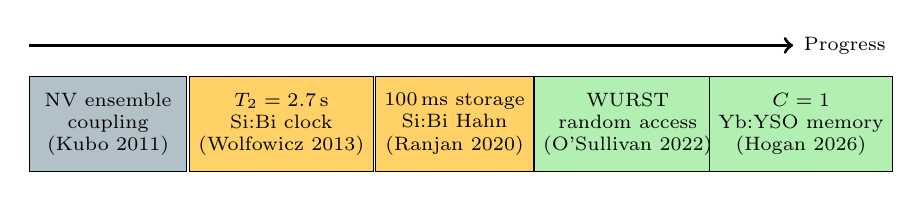
\begin{tikzpicture}[every node/.style={font=\scriptsize, align=center}]
        \draw[->, very thick] (0,1) -- (9.7,1) node[right] {Progress};
        \node[draw, fill=lightgray, minimum width=2.0cm, minimum height=1.2cm] at (1,0)
            {NV ensemble\\coupling\\(Kubo 2011)};
        \node[draw, fill=lightorange, minimum width=2.0cm, minimum height=1.2cm] at (3.2,0)
            {$T_2 = 2.7$\,s\\Si:Bi clock\\(Wolfowicz 2013)};
        \node[draw, fill=lightorange, minimum width=2.0cm, minimum height=1.2cm] at (5.4,0)
            {100\,ms storage\\Si:Bi Hahn\\(Ranjan 2020)};
        \node[draw, fill=paleGreen, minimum width=2.0cm, minimum height=1.2cm] at (7.6,0)
            {WURST\\random access\\(O'Sullivan 2022)};
        \node[draw, fill=paleGreen, minimum width=2cm, minimum height=1.2cm] at (9.8,0)
            {$C=1$\\Yb:YSO memory\\(Hogan 2026)};
    \end{tikzpicture}%
    }
    \end{center}

    \vspace{0.05cm}
    \begin{itemize}
        \item<2-> Clock-transition engineering in Si:Bi pushes $T_2 > 1$\,s
        \item<3-> WURST delivers random access, natural dynamical decoupling
        \item<4-> Unit cooperativity achieved in Yb:YSO memories; efficiency now limited by surrounding circuit
        \item<5-> \textbf{Remaining challenges:} unit $C$ $\to$ unit efficiency in a fully integrated device + increased mode count
        \item<6-> \textbf{Long-term:} integration of microwave spin memories into fibre-optical quantum networks
    \end{itemize}
\end{frame}

% THANK YOU ==================================================
\begin{frame}[standout]
    Thank you for listening!
\end{frame}

\end{document}
